%!TEX root = ../thesis.tex
% Spellchecker ignore
% cSpell:ignore redbluedetuning, trapdepth, giga, detuningopt, cmmnt, waals, potentialoverlap, eqref, dipolepot, wrapfigure, intensityplot, includegraphics, retroreflected, detunings, linewidth, dispersive, antinodes, pagebreak, ifpdf, graphicspath, detuned, bigskip, nano, citep, milli, detuning, medskip, mathrm
%*******************************************************************************
%****************************** First Chapter **********************************
%*******************************************************************************

\chapter{\label{chap:dipole}Theory of laser trapping of atoms}


\ifpdf{}
    \graphicspath{{Chapter1/Figs/Raster/}{Chapter1/Figs/PDF/}{Chapter1/Figs/}}
\else
    \graphicspath{{Chapter1/Figs/Vector/}{Chapter1/Figs/}}
\fi

\begin{wrapfigure}{R}{.4\textwidth}
    \centering
    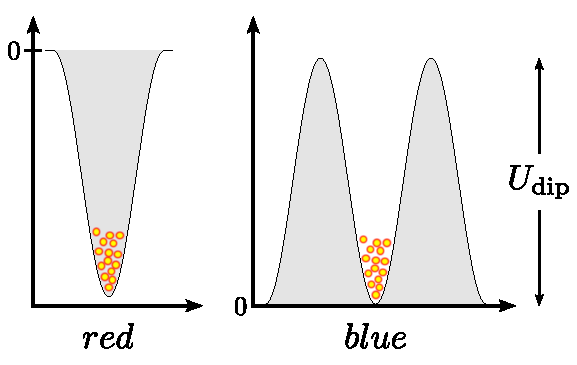
\includegraphics[width=0.35\textwidth]{redbluedetuning}    
    \caption{\label{fig:redbluedetuning} Illustration of dipole traps with red and blue detuning.}
\end{wrapfigure}
Atoms can be trapped in a optical potential created by the dispersive interaction of 
the atomic dipole moment with the intensity gradient of the light field. These trap 
can be used to confine the atoms in 3D, and to counter gravity. In the case of large 
detunings the expression for the dipole potential and scattering rate~\cite{grimm} is 
the following:
%
\begin{align} \label{eq:dipolepot_simple}
    U_\mathrm{dip}(z) =& \frac{3\pi c^2}{2\omega_0^3}~\frac{\Gamma}{\Delta}~I(z)~, \\
    \Gamma_{\mathrm{sc}}(z) =& \frac{3\pi c^2}{2\hbar\omega_0^3}~
    {\left ( \frac{\Gamma}{\Delta} \right )}^2~I(z)~.
\end{align}
%
Where \textit{c} is the speed of light, \(\Gamma \) is the transition rate for 
an atom in the excited state to decay to the
ground state, \(\omega_0=2\pi~\frac{c}{\lambda}=2\pi\nu \), \(\Delta \) 
is the detuning between the light and the atomic transition (\(\Delta := \omega - \omega_0 \)), 
where \(\omega \) is the driving frequency of the light field and \(I(z) \) 
corresponds to the intensity at a given distance to the resonator. Dipole traps can 
be divided into two main classes, red-detuned traps (``red'' detuning, \(\Delta < 0 \)) 
and blue-detuned traps (``blue'' detuning, \(\Delta > 0 \)). Below an atomic resonance the dipole potential is
negative and the potential minima are therefore found at positions with maximum 
intensity and potential minima correspond to minima of the intensity and the
??? repels atoms from the field??? as seen in Fig.~\ref{fig:redbluedetuning}.\\

For our case there are three different red-detuned trap configurations possible: 
\textit{Focused-beam traps} consisting of a single beam, the
\textit{crossed-beam traps} created by two or more beams intersecting at their foci,
and \textit{standing-wave traps} where atoms are axially confined in the antinodes
of a standing wave.
For our Experiment it is important that the atoms are as close as possible from the
resonator, because the interacting evanescent field of the photon in the resonator
decreases exponentially with a decay length of \(\frac{\lambda_{at} }{2\pi} \) where 
\(\lambda_{at} \) is the wavelength of the atomic transition. \SI{780}{\nano\meter}
for the \(D_2 \) line \(5S_{1/2} \rightarrow 5P_{3/2} \) of Rb.\\

\begin{wrapfigure}{R}{.4\textwidth}
    \centering
    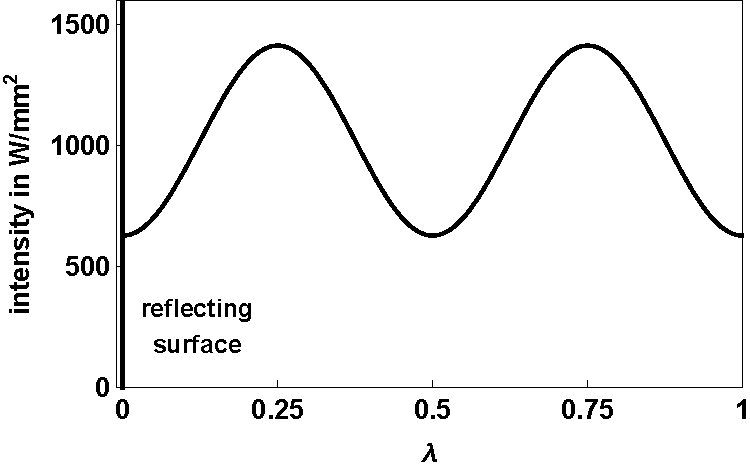
\includegraphics[width=0.35\textwidth]{intensityplot}    
    \caption{\label{fig:intensityplot} 1D Intensity distribution of a retroreflected gaussian laser beam. }
\end{wrapfigure}
The closest trap potential provides a retroreflected gaussian beam with a distance
of \(\frac{\lambda_{laser}}{4} \) at the first minimum of the standing wave 
(see Fig.~\ref{fig:intensityplot}). If one
uses a laser closely detuned from the \(D_2 \) line \(5S_{1/2} \rightarrow 5P_{3/2} \), 
i.e. @ \SI{783}{\nano\meter}, which leads to a distance of 
\(\frac{\lambda}{4} \approx \SI{190}{\nano\meter} \), but this would be to far from
the resonator. For rubidium it is possible to 
use alternatively a laser close to the \(5S_{1/2} \rightarrow 6P_{3/2} \) @ \SI{420}{\nano\meter}, 
this would reduce the distance to the resonator to \SI{105}{\nano\meter}. \\
As we can see in~\eqref{eq:dipolepot_simple} the dipole potential is 
\(\sim \frac{I}{\Delta} \). To condition our setup properly we have to consider some
constraints. Laser power is limited and additionally we do not want to send too
much power onto the resonator, because of safety precautions. On the other hand we
want to keep the scattering rate as low as possible, which is \(\sim \frac{I}{\Delta^2} \).
However if \(\Delta < \) separation between \(D_1 \) \& \(D_2 \) lines (\SI{420} \& \SI{421}{\nano\meter}) then we need to take the fine 
structure into account and for that equation~\eqref{eq:dipolepot_simple} isn't sufficient enough. In our case we are 
red-detuned from the \(D_2 \)-transition and the detuning will be smaller than the fine 
structure splitting of \SI{2.32}{\tera\hertz}, so we get an additional counter term 
of the \(D_1 \)-transition (blue-detuned):
%
\begin{align}
    U_\mathrm{dip}(z) =& \frac{\pi c^2}{2\omega_0^3}~\left( 
        \frac{2~\Gamma_{\omega,D2}}{\Delta_{D2}} + 
        \frac{\Gamma_{\omega,D1}}{\Delta_{D1}} \right)~I(z)~, \\
    \Gamma_{\mathrm{sc}}(z) =& \frac{\pi c^2}{2\hbar\omega_0^3}~\left( 
        \frac{2~\Gamma_{\omega,D2}~\Gamma_{\omega,D2,tot} }{\Delta_{D2}^2 } + 
        \frac{\Gamma_{\omega,D1}~\Gamma_{\omega,D1,tot} }{\Delta_{D1}^2 } \right)~I(z)~.
\end{align}
%
% TODO: Add explanation of the factor of 2 in above equation and why in the original equation is only one Gamma
\(\Gamma_{\omega,Dx} \) are the transition rates from \(6P_{1/2} \) for the \(D_1 \) line 
and accordantly \(6P_{3/2} \) for the \(D_2 \) line to decay to \(5S_{1/2} \), 
\(\Gamma_{\omega,Dx,tot} \) are the transition rates from \(6P_{1/2} \& 6P_{3/2} \) over
all their decay channels with \(\frac{1}{\Gamma_{\omega,Dx,tot}} \) is the mean lifetime
of the state and \(\Delta_{Dx} \) represents \(\omega - \omega_{0,Dx} \).
All values can be found in table~\ref{table:iso_prop}. 
\pagebreak

\subsection*{Possible configuration of optical dipole trap}
\begin{figure}[h]
    \centering
    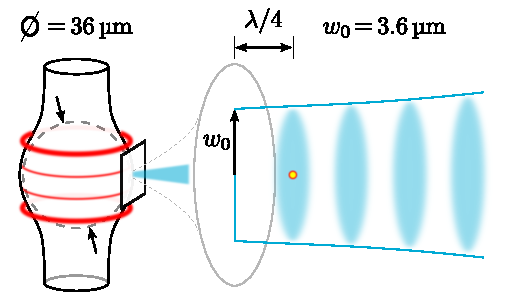
\includegraphics[width=0.6\textwidth]{resonator_trap_label}
    \caption{\label{fig:resonator_trap_label} Experimental setup and intensity distribution. }
\end{figure}
\begin{wrapfigure}{RH}{.4\textwidth}
    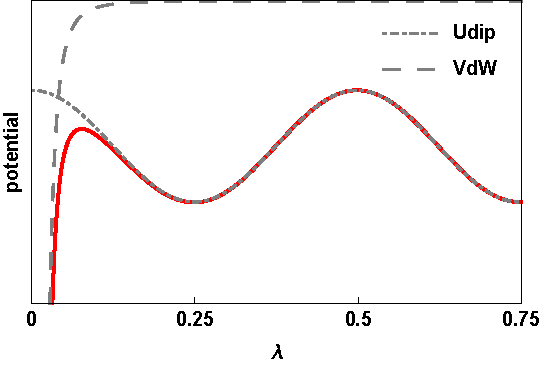
\includegraphics[width=0.35\textwidth]{potentialoverlap}    
    \caption{\label{fig:potentialoverlap} Overlap of Dipole and Van-der-Waals potential.}
    \vspace{2em}
    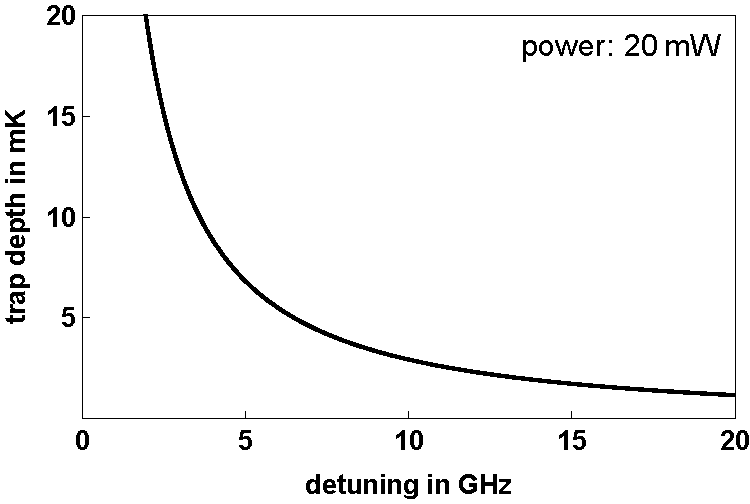
\includegraphics[width=0.35\textwidth]{detuningopt}    
    \caption{\label{fig:detuningopt} Trap depth for different detuning.}
    \vspace{2em}
    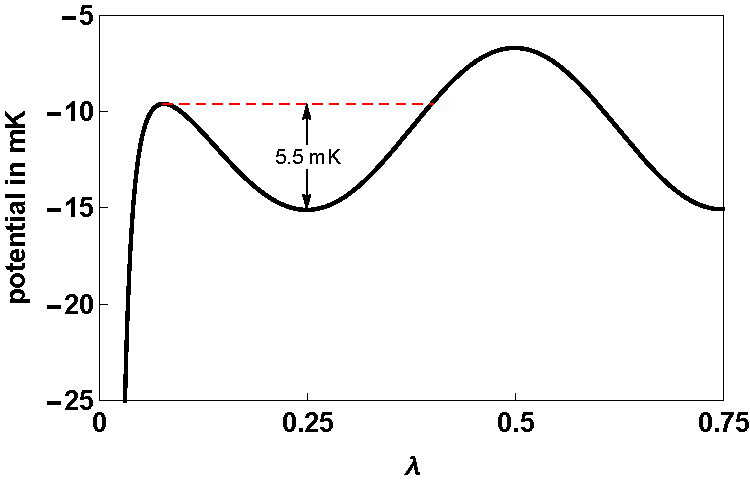
\includegraphics[width=0.35\textwidth]{trapdepth}    
    \caption{\label{fig:trapdepth} Calculated trap potential for \SI{20}{\milli\watt} power and a \SI{6}{\giga\hertz} detuning.}
\end{wrapfigure}
Our goal is to trap the free falling atoms as close as possible to the resonator by
simultaneously low scattering rate and without damaging the resonator with the incoming
laser beam. To calculate the trap potential we have to derive the intensity for a
gaussian beam, but to get the intensity one has to calculate the electric field first.
One considers that the beam is enough focused on the resonator that the reflecting
surface is more or less ``flat'' (see Fig.~\ref{fig:resonator_trap_label}). With this 
assumption the electric field becomes:
\begin{align}
    \hat{E}(z) = \hat{x}~\left( e^{-i k_z z} + r e^{i k_z z} \right)
\end{align}
with \(r \) as the reflection coefficient, which is in case of our resonator surface
\(r = -0.02 \). This leads to the intensity:
\begin{align}
    I(z) = \frac{ { | \hat{E}(z) | }^2}{2\eta} =
    I_0 \left [ 1 + r^2 + 2r \cos{\left( \frac{2\omega}{c}~z \right) } \right ]~.
\end{align}
Where \(I_0 = \frac{{E_0}^2}{2\eta} \) and \(\omega \) is the driving frequency of the
laser. For further calculation we need the dipole potential dependent from the laser power.
The power of a gaussian beam is defined as:
\begin{align}
    P_0 = \frac{1}{2}~I_0 {w_0}^2 \pi
\end{align} 
with \(w_0 \) as the beam radius, which is for our setup \(w_0 = \SI{3.6}{\micro\meter} \) 
as pictured in Fig.~\ref{fig:resonator_trap_label}.
To have only one parameter to adjust we will choose a power between 
\(0~<~P~<\SI{80}{\milli\watt} \). The trap depth must be bigger than the energy of the
atom, here the kinetic energy \(E_{kin} = \frac{1}{2}m_{Rb} v^2 \) due to the fact that 
the atoms are free falling for between \SI{0} and \SI{60}{\milli\second} would be in terms of temperature 
\(E_{kin}/k_B = \SI{1.77}{\milli\kelvin} \). Our trap without cooling 
is conservative, this means the captured atoms keep there energy. If now an
atom is not captured in the middle of the potential well it gains additional 
potential energy and it's total energy increases. It is then possible that
the atom can escape the trap. Therefore one should add a safety margin to
capture more atoms. For example a \SI{5}{\milli\kelvin} trap would capture
 \(\frac{5-1.77}{5}~\SI{100}{\percent} \approx \SI{60}{\percent} \) 
of atoms entering the trap in the worst case, because atoms have
\(E_{kin}/k_B < \SI{1.77}{\milli\kelvin} \).
In our setup we are so close to the resonator that we have to consider a Van-der-Waals 
potential, which reduces our first potential barrier (see Fig.~\ref{fig:potentialoverlap}).\\

To determine a correct detuning for our trap we will use the combination of both 
potentials in all further calculations. The depth of the potential well is now
the difference between the reduced first maximum and the first minimum at
\(\lambda/4 \). As we can see in Fig.~\ref{fig:detuningopt}
the detuning has to be lower than \SI{7}{\giga\hertz}. For a detuning of \SI{6}{\giga\hertz}
we get a trap depth of \SI{5.5}{\milli\kelvin} as shown in Fig.~\ref{fig:trapdepth}~.  
  





\pagebreak

This requires to see the transitions to have a reference to lock the laser afterwards.
\bigskip
To determine \(\Gamma_{\omega,420nm-Line} \) we can use a theoretical relation with the intensity saturation, which has to be checked by our measurement:
\begin{align}
    I_{s,420} &= \frac{\Gamma_{\omega,tot,420}\cdot{\omega_{420}}^3\cdot I_{s,780}}{\Gamma_{\omega,420}\cdot\Gamma_{\omega,780}\cdot{\omega_{780}}^3}
\end{align}
\begin{align*}
    \text{with~~~} \Gamma_{\omega,tot,420} &= \frac{1}{total~lifetime~of~6P_{3/2}~state}
\end{align*}
\medskip


\(\Rightarrow \) We want to measure \(I_{s}\) for the blue \SI{420.29}{\nano\meter}-line. 

